\documentclass{standalone}
\usepackage{graphicx}	
\usepackage{amssymb, amsmath, amsthm}
\usepackage{color}

\usepackage{tikz}
\usetikzlibrary{intersections, backgrounds}

\definecolor{light}{RGB}{220, 188, 188}
\definecolor{mid}{RGB}{185, 124, 124}
\definecolor{dark}{RGB}{143, 39, 39}
\definecolor{highlight}{RGB}{180, 31, 180}
\definecolor{gray10}{gray}{0.1}
\definecolor{gray20}{gray}{0.2}
\definecolor{gray30}{gray}{0.3}
\definecolor{gray40}{gray}{0.4}
\definecolor{gray60}{gray}{0.6}
\definecolor{gray70}{gray}{0.7}
\definecolor{gray80}{gray}{0.8}
\definecolor{gray90}{gray}{0.9}
\definecolor{gray60}{gray}{0.95}

\begin{document}

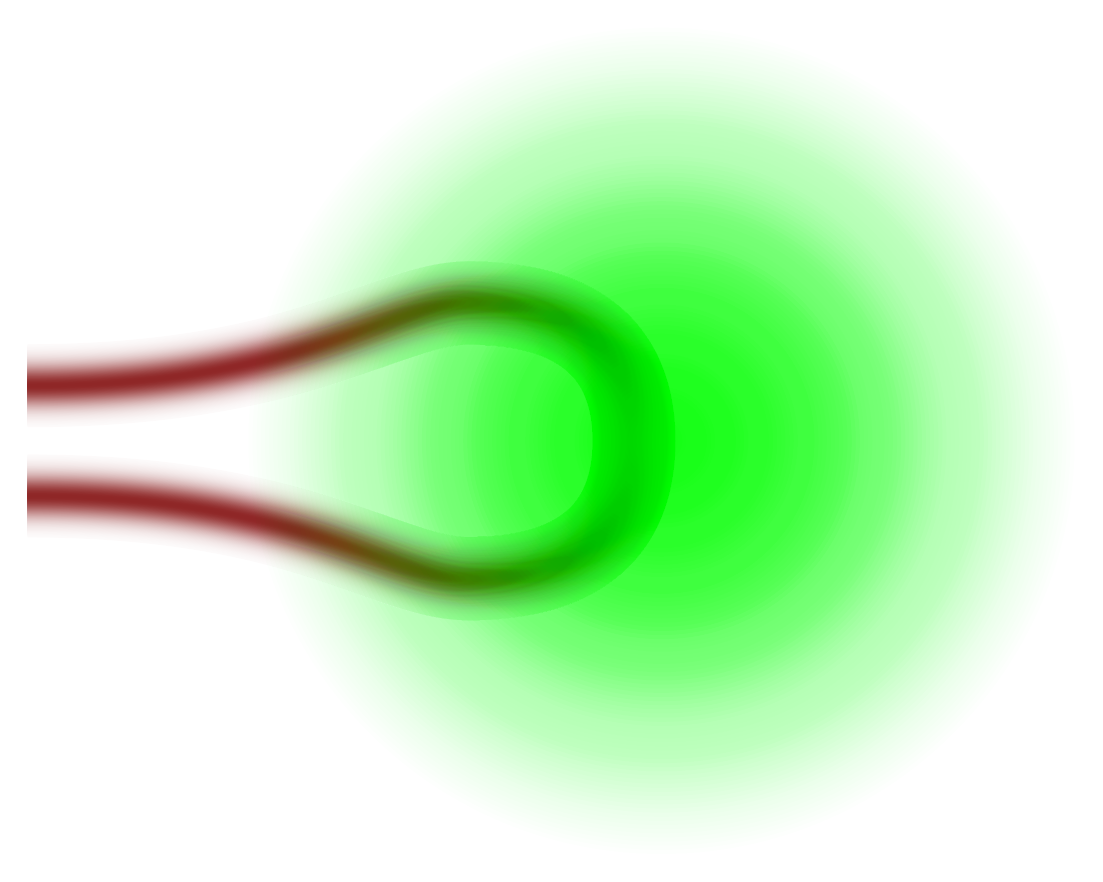
\begin{tikzpicture}[scale=0.35, thick]
  \begin{scope}
    \clip (-12, -6) rectangle (12, 10);
    \foreach \i in {1, 0.99, ..., 0} {
      \pgfmathsetmacro{\prop}{100 * exp(-4.0 * \i * \i)};
      \colorlet{custom}{dark!\prop!white};
      \draw[line width={30 * \i}, color=custom] 
        (-12, 3)
        .. controls (-2, 3) and (1, 6) .. (4, 6) 
        .. controls (7, 6) and (10, 5) .. (10, 1) 
        .. controls (10, -3) and (7, -4) .. (4, -4) 
        .. controls (1, -4) and (-2, -1) .. 
        (-12, -1);
    }  
  \end{scope}
  
  \pgfmathsetmacro{\x}{10.5}
  \pgfmathsetmacro{\y}{1}
  \pgfmathsetmacro{\delta}{2}
  \foreach \i in {0, 0.01,..., 1} {
    \fill[color=green, opacity={0.05 * exp(-2 * \i * \i)}]
      (11, 1) circle ({15 * \i});
  }
\end{tikzpicture}

\end{document}  